\documentclass[1p]{elsarticle_modified}
%\bibliographystyle{elsarticle-num}

%\usepackage[colorlinks]{hyperref}
%\usepackage{abbrmath_seonhwa} %\Abb, \Ascr, \Acal ,\Abf, \Afrak
\usepackage{amsfonts}
\usepackage{amssymb}
\usepackage{amsmath}
\usepackage{amsthm}
\usepackage{scalefnt}
\usepackage{amsbsy}
\usepackage{kotex}
\usepackage{caption}
\usepackage{subfig}
\usepackage{color}
\usepackage{graphicx}
\usepackage{xcolor} %% white, black, red, green, blue, cyan, magenta, yellow
\usepackage{float}
\usepackage{setspace}
\usepackage{hyperref}

\usepackage{tikz}
\usetikzlibrary{arrows}

\usepackage{multirow}
\usepackage{array} % fixed length table
\usepackage{hhline}

%%%%%%%%%%%%%%%%%%%%%
\makeatletter
\renewcommand*\env@matrix[1][\arraystretch]{%
	\edef\arraystretch{#1}%
	\hskip -\arraycolsep
	\let\@ifnextchar\new@ifnextchar
	\array{*\c@MaxMatrixCols c}}
\makeatother %https://tex.stackexchange.com/questions/14071/how-can-i-increase-the-line-spacing-in-a-matrix
%%%%%%%%%%%%%%%

\usepackage[normalem]{ulem}

\newcommand{\msout}[1]{\ifmmode\text{\sout{\ensuremath{#1}}}\else\sout{#1}\fi}
%SOURCE: \msout is \stkout macro in https://tex.stackexchange.com/questions/20609/strikeout-in-math-mode

\newcommand{\cancel}[1]{
	\ifmmode
	{\color{red}\msout{#1}}
	\else
	{\color{red}\sout{#1}}
	\fi
}

\newcommand{\add}[1]{
	{\color{blue}\uwave{#1}}
}

\newcommand{\replace}[2]{
	\ifmmode
	{\color{red}\msout{#1}}{\color{blue}\uwave{#2}}
	\else
	{\color{red}\sout{#1}}{\color{blue}\uwave{#2}}
	\fi
}

\newcommand{\Sol}{\mathcal{S}} %segment
\newcommand{\D}{D} %diagram
\newcommand{\A}{\mathcal{A}} %arc


%%%%%%%%%%%%%%%%%%%%%%%%%%%%%5 test

\def\sl{\operatorname{\textup{SL}}(2,\Cbb)}
\def\psl{\operatorname{\textup{PSL}}(2,\Cbb)}
\def\quan{\mkern 1mu \triangleright \mkern 1mu}

\theoremstyle{definition}
\newtheorem{thm}{Theorem}[section]
\newtheorem{prop}[thm]{Proposition}
\newtheorem{lem}[thm]{Lemma}
\newtheorem{ques}[thm]{Question}
\newtheorem{cor}[thm]{Corollary}
\newtheorem{defn}[thm]{Definition}
\newtheorem{exam}[thm]{Example}
\newtheorem{rmk}[thm]{Remark}
\newtheorem{alg}[thm]{Algorithm}

\newcommand{\I}{\sqrt{-1}}
\begin{document}

%\begin{frontmatter}
%
%\title{Boundary parabolic representations of knots up to 8 crossings}
%
%%% Group authors per affiliation:
%\author{Yunhi Cho} 
%\address{Department of Mathematics, University of Seoul, Seoul, Korea}
%\ead{yhcho@uos.ac.kr}
%
%
%\author{Seonhwa Kim} %\fnref{s_kim}}
%\address{Center for Geometry and Physics, Institute for Basic Science, Pohang, 37673, Korea}
%\ead{ryeona17@ibs.re.kr}
%
%\author{Hyuk Kim}
%\address{Department of Mathematical Sciences, Seoul National University, Seoul 08826, Korea}
%\ead{hyukkim@snu.ac.kr}
%
%\author{Seokbeom Yoon}
%\address{Department of Mathematical Sciences, Seoul National University, Seoul, 08826,  Korea}
%\ead{sbyoon15@snu.ac.kr}
%
%\begin{abstract}
%We find all boundary parabolic representation of knots up to 8 crossings.
%
%\end{abstract}
%\begin{keyword}
%    \MSC[2010] 57M25 
%\end{keyword}
%
%\end{frontmatter}

%\linenumbers
%\tableofcontents
%
\newcommand\colored[1]{\textcolor{white}{\rule[-0.35ex]{0.8em}{1.4ex}}\kern-0.8em\color{red} #1}%
%\newcommand\colored[1]{\textcolor{white}{ #1}\kern-2.17ex	\textcolor{white}{ #1}\kern-1.81ex	\textcolor{white}{ #1}\kern-2.15ex\color{red}#1	}

{\Large $\underline{12n_{0709}~(K12n_{0709})}$}

\setlength{\tabcolsep}{10pt}
\renewcommand{\arraystretch}{1.6}
\vspace{1cm}\begin{tabular}{m{100pt}>{\centering\arraybackslash}m{274pt}}
\multirow{5}{120pt}{
	\centering
	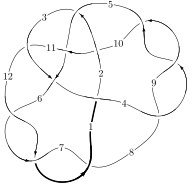
\includegraphics[width=112pt]{../../../GIT/diagram.site/Diagrams/png/2798_12n_0709.png}\\
\ \ \ A knot diagram\footnotemark}&
\allowdisplaybreaks
\textbf{Linearized knot diagam} \\
\cline{2-2}
 &
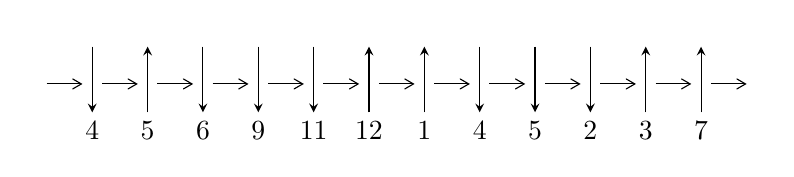
\begin{tikzpicture}[x=20pt, y=17pt]
	% nodes
	\node (C0) at (0, 0) {};
	\node (C1) at (1, 0) {};
	\node (C1U) at (1, +1) {};
	\node (C1D) at (1, -1) {4};

	\node (C2) at (2, 0) {};
	\node (C2U) at (2, +1) {};
	\node (C2D) at (2, -1) {5};

	\node (C3) at (3, 0) {};
	\node (C3U) at (3, +1) {};
	\node (C3D) at (3, -1) {6};

	\node (C4) at (4, 0) {};
	\node (C4U) at (4, +1) {};
	\node (C4D) at (4, -1) {9};

	\node (C5) at (5, 0) {};
	\node (C5U) at (5, +1) {};
	\node (C5D) at (5, -1) {11};

	\node (C6) at (6, 0) {};
	\node (C6U) at (6, +1) {};
	\node (C6D) at (6, -1) {12};

	\node (C7) at (7, 0) {};
	\node (C7U) at (7, +1) {};
	\node (C7D) at (7, -1) {1};

	\node (C8) at (8, 0) {};
	\node (C8U) at (8, +1) {};
	\node (C8D) at (8, -1) {4};

	\node (C9) at (9, 0) {};
	\node (C9U) at (9, +1) {};
	\node (C9D) at (9, -1) {5};

	\node (C10) at (10, 0) {};
	\node (C10U) at (10, +1) {};
	\node (C10D) at (10, -1) {2};

	\node (C11) at (11, 0) {};
	\node (C11U) at (11, +1) {};
	\node (C11D) at (11, -1) {3};

	\node (C12) at (12, 0) {};
	\node (C12U) at (12, +1) {};
	\node (C12D) at (12, -1) {7};
	\node (C13) at (13, 0) {};

	% arrows
	\draw[->,>={angle 60}]
	(C0) edge (C1) (C1) edge (C2) (C2) edge (C3) (C3) edge (C4) (C4) edge (C5) (C5) edge (C6) (C6) edge (C7) (C7) edge (C8) (C8) edge (C9) (C9) edge (C10) (C10) edge (C11) (C11) edge (C12) (C12) edge (C13) ;	\draw[->,>=stealth]
	(C1U) edge (C1D) (C2D) edge (C2U) (C3U) edge (C3D) (C4U) edge (C4D) (C5U) edge (C5D) (C6D) edge (C6U) (C7D) edge (C7U) (C8U) edge (C8D) (C9U) edge (C9D) (C10U) edge (C10D) (C11D) edge (C11U) (C12D) edge (C12U) ;
	\end{tikzpicture} \\
\hhline{~~} \\& 
\textbf{Solving Sequence} \\ \cline{2-2} 
 &
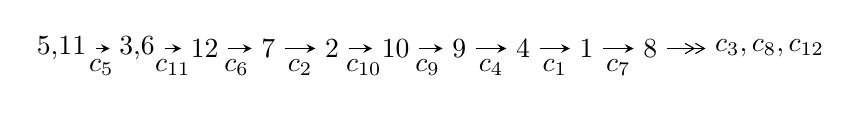
\begin{tikzpicture}[x=23pt, y=7pt]
	% node
	\node (A0) at (-1/8, 0) {5,11};
	\node (A1) at (17/16, 0) {3,6};
	\node (A2) at (17/8, 0) {12};
	\node (A3) at (25/8, 0) {7};
	\node (A4) at (33/8, 0) {2};
	\node (A5) at (41/8, 0) {10};
	\node (A6) at (49/8, 0) {9};
	\node (A7) at (57/8, 0) {4};
	\node (A8) at (65/8, 0) {1};
	\node (A9) at (73/8, 0) {8};
	\node (C1) at (1/2, -1) {$c_{5}$};
	\node (C2) at (13/8, -1) {$c_{11}$};
	\node (C3) at (21/8, -1) {$c_{6}$};
	\node (C4) at (29/8, -1) {$c_{2}$};
	\node (C5) at (37/8, -1) {$c_{10}$};
	\node (C6) at (45/8, -1) {$c_{9}$};
	\node (C7) at (53/8, -1) {$c_{4}$};
	\node (C8) at (61/8, -1) {$c_{1}$};
	\node (C9) at (69/8, -1) {$c_{7}$};
	\node (A10) at (11, 0) {$c_{3},c_{8},c_{12}$};

	% edge
	\draw[->,>=stealth]	
	(A0) edge (A1) (A1) edge (A2) (A2) edge (A3) (A3) edge (A4) (A4) edge (A5) (A5) edge (A6) (A6) edge (A7) (A7) edge (A8) (A8) edge (A9) ;
	\draw[->>,>={angle 60}]	
	(A9) edge (A10);
\end{tikzpicture} \\ 

\end{tabular} \\

\footnotetext{
The image of knot diagram is generated by the software ``\textbf{Draw programme}" developed by Andrew Bartholomew(\url{http://www.layer8.co.uk/maths/draw/index.htm\#Running-draw}), where we modified some parts for our purpose(\url{https://github.com/CATsTAILs/LinksPainter}).
}\phantom \\ \newline 
\centering \textbf{Ideals for irreducible components\footnotemark of $X_{\text{par}}$} 
 
\begin{align*}
I^u_{1}&=\langle 
4.82508\times10^{67} u^{41}-8.04373\times10^{66} u^{40}+\cdots+3.17613\times10^{68} b+7.49719\times10^{68},\\
\phantom{I^u_{1}}&\phantom{= \langle  }7.68981\times10^{68} u^{41}+6.83382\times10^{67} u^{40}+\cdots+3.17613\times10^{68} a+4.36130\times10^{69},\;u^{42}-5 u^{40}+\cdots+12 u-1\rangle \\
I^u_{2}&=\langle 
2 u^{11}+2 u^{10}-9 u^9-9 u^8+17 u^7+11 u^6-20 u^5-5 u^4+14 u^3+5 u^2+b-3 u,\\
\phantom{I^u_{2}}&\phantom{= \langle  }3 u^{11}+4 u^{10}-13 u^9-19 u^8+23 u^7+30 u^6-27 u^5-26 u^4+21 u^3+22 u^2+a-5 u-6,\\
\phantom{I^u_{2}}&\phantom{= \langle  }u^{12}+u^{11}-5 u^{10}-5 u^9+11 u^8+8 u^7-15 u^6-6 u^5+13 u^4+4 u^3-6 u^2- u+1\rangle \\
\\
\end{align*}
\raggedright * 2 irreducible components of $\dim_{\mathbb{C}}=0$, with total 54 representations.\\
\footnotetext{All coefficients of polynomials are rational numbers. But the coefficients are sometimes approximated in decimal forms when there is not enough margin.}
\newpage
\renewcommand{\arraystretch}{1}
\centering \section*{I. $I^u_{1}= \langle 4.83\times10^{67} u^{41}-8.04\times10^{66} u^{40}+\cdots+3.18\times10^{68} b+7.50\times10^{68},\;7.69\times10^{68} u^{41}+6.83\times10^{67} u^{40}+\cdots+3.18\times10^{68} a+4.36\times10^{69},\;u^{42}-5 u^{40}+\cdots+12 u-1 \rangle$}
\flushleft \textbf{(i) Arc colorings}\\
\begin{tabular}{m{7pt} m{180pt} m{7pt} m{180pt} }
\flushright $a_{5}=$&$\begin{pmatrix}1\\0\end{pmatrix}$ \\
\flushright $a_{11}=$&$\begin{pmatrix}0\\u\end{pmatrix}$ \\
\flushright $a_{3}=$&$\begin{pmatrix}-2.42113 u^{41}-0.215162 u^{40}+\cdots+47.7375 u-13.7315\\-0.151917 u^{41}+0.0253256 u^{40}+\cdots+4.43664 u-2.36048\end{pmatrix}$ \\
\flushright $a_{6}=$&$\begin{pmatrix}1\\u^2\end{pmatrix}$ \\
\flushright $a_{12}=$&$\begin{pmatrix}1.40883 u^{41}-0.283645 u^{40}+\cdots-31.6002 u+11.3295\\0.451792 u^{41}-0.229337 u^{40}+\cdots+0.897332 u+1.83430\end{pmatrix}$ \\
\flushright $a_{7}=$&$\begin{pmatrix}-1.66145 u^{41}-0.892224 u^{40}+\cdots+72.0897 u-18.1638\\0.208120 u^{41}-0.395827 u^{40}+\cdots+17.3792 u-4.31286\end{pmatrix}$ \\
\flushright $a_{2}=$&$\begin{pmatrix}-2.26921 u^{41}-0.240488 u^{40}+\cdots+43.3008 u-11.3710\\-0.151917 u^{41}+0.0253256 u^{40}+\cdots+4.43664 u-2.36048\end{pmatrix}$ \\
\flushright $a_{10}=$&$\begin{pmatrix}0.699121 u^{41}-0.0570474 u^{40}+\cdots-24.8728 u+7.43404\\0.257913 u^{41}+0.00273987 u^{40}+\cdots-5.62471 u+2.06112\end{pmatrix}$ \\
\flushright $a_{9}=$&$\begin{pmatrix}0.957035 u^{41}-0.0543075 u^{40}+\cdots-30.4975 u+9.49516\\0.257913 u^{41}+0.00273987 u^{40}+\cdots-5.62471 u+2.06112\end{pmatrix}$ \\
\flushright $a_{4}=$&$\begin{pmatrix}-2.53284 u^{41}-0.147464 u^{40}+\cdots+43.4617 u-11.5862\\-0.325011 u^{41}+0.129277 u^{40}+\cdots+3.51256 u-2.29278\end{pmatrix}$ \\
\flushright $a_{1}=$&$\begin{pmatrix}-2.13070 u^{41}-0.169775 u^{40}+\cdots+38.9427 u-12.7081\\-0.812419 u^{41}+0.186428 u^{40}+\cdots+8.64257 u-3.43916\end{pmatrix}$ \\
\flushright $a_{8}=$&$\begin{pmatrix}-0.374567 u^{41}+0.0574880 u^{40}+\cdots+18.7871 u+0.721860\\0.269350 u^{41}+0.303079 u^{40}+\cdots-12.4553 u+2.13098\end{pmatrix}$\\&\end{tabular}
\flushleft \textbf{(ii) Obstruction class $= -1$}\\~\\
\flushleft \textbf{(iii) Cusp Shapes $= 0.117845 u^{41}-0.341047 u^{40}+\cdots-3.69676 u+5.23841$}\\~\\
\newpage\renewcommand{\arraystretch}{1}
\flushleft \textbf{(iv) u-Polynomials at the component}\newline \\
\begin{tabular}{m{50pt}|m{274pt}}
Crossings & \hspace{64pt}u-Polynomials at each crossing \\
\hline $$\begin{aligned}c_{1}\end{aligned}$$&$\begin{aligned}
&u^{42}-2 u^{41}+\cdots+7155 u+1759
\end{aligned}$\\
\hline $$\begin{aligned}c_{2}\end{aligned}$$&$\begin{aligned}
&u^{42}-20 u^{40}+\cdots-4 u+1
\end{aligned}$\\
\hline $$\begin{aligned}c_{3}\end{aligned}$$&$\begin{aligned}
&u^{42}-3 u^{40}+\cdots+36 u-7
\end{aligned}$\\
\hline $$\begin{aligned}c_{4},c_{8},c_{9}\end{aligned}$$&$\begin{aligned}
&u^{42}- u^{41}+\cdots+125 u-43
\end{aligned}$\\
\hline $$\begin{aligned}c_{5}\end{aligned}$$&$\begin{aligned}
&u^{42}-5 u^{40}+\cdots+12 u-1
\end{aligned}$\\
\hline $$\begin{aligned}c_{6},c_{7},c_{12}\end{aligned}$$&$\begin{aligned}
&u^{42}-2 u^{41}+\cdots-9 u+1
\end{aligned}$\\
\hline $$\begin{aligned}c_{10}\end{aligned}$$&$\begin{aligned}
&u^{42}+u^{41}+\cdots+17 u+1
\end{aligned}$\\
\hline $$\begin{aligned}c_{11}\end{aligned}$$&$\begin{aligned}
&u^{42}-2 u^{41}+\cdots-260 u-29
\end{aligned}$\\
\hline
\end{tabular}\\~\\
\newpage\renewcommand{\arraystretch}{1}
\flushleft \textbf{(v) Riley Polynomials at the component}\newline \\
\begin{tabular}{m{50pt}|m{274pt}}
Crossings & \hspace{64pt}Riley Polynomials at each crossing \\
\hline $$\begin{aligned}c_{1}\end{aligned}$$&$\begin{aligned}
&y^{42}+84 y^{41}+\cdots-28548659 y+3094081
\end{aligned}$\\
\hline $$\begin{aligned}c_{2}\end{aligned}$$&$\begin{aligned}
&y^{42}-40 y^{41}+\cdots-132 y+1
\end{aligned}$\\
\hline $$\begin{aligned}c_{3}\end{aligned}$$&$\begin{aligned}
&y^{42}-6 y^{41}+\cdots-246 y+49
\end{aligned}$\\
\hline $$\begin{aligned}c_{4},c_{8},c_{9}\end{aligned}$$&$\begin{aligned}
&y^{42}+5 y^{41}+\cdots+3123 y+1849
\end{aligned}$\\
\hline $$\begin{aligned}c_{5}\end{aligned}$$&$\begin{aligned}
&y^{42}-10 y^{41}+\cdots-102 y+1
\end{aligned}$\\
\hline $$\begin{aligned}c_{6},c_{7},c_{12}\end{aligned}$$&$\begin{aligned}
&y^{42}-56 y^{41}+\cdots-185 y+1
\end{aligned}$\\
\hline $$\begin{aligned}c_{10}\end{aligned}$$&$\begin{aligned}
&y^{42}+41 y^{41}+\cdots-193 y+1
\end{aligned}$\\
\hline $$\begin{aligned}c_{11}\end{aligned}$$&$\begin{aligned}
&y^{42}-26 y^{41}+\cdots-54028 y+841
\end{aligned}$\\
\hline
\end{tabular}\\~\\
\newpage\flushleft \textbf{(vi) Complex Volumes and Cusp Shapes}
$$\begin{array}{c|c|c}  
\text{Solutions to }I^u_{1}& \I (\text{vol} + \sqrt{-1}CS) & \text{Cusp shape}\\
 \hline 
\begin{aligned}
u &= -0.826491 + 0.442043 I \\
a &= \phantom{-}0.44718 + 1.76659 I \\
b &= \phantom{-}0.70153 + 1.70890 I\end{aligned}
 & \phantom{-}7.45710 + 5.86314 I & -2.65176 - 8.52020 I \\ \hline\begin{aligned}
u &= -0.826491 - 0.442043 I \\
a &= \phantom{-}0.44718 - 1.76659 I \\
b &= \phantom{-}0.70153 - 1.70890 I\end{aligned}
 & \phantom{-}7.45710 - 5.86314 I & -2.65176 + 8.52020 I \\ \hline\begin{aligned}
u &= -0.922502\phantom{ +0.000000I} \\
a &= -1.78773\phantom{ +0.000000I} \\
b &= -0.148859\phantom{ +0.000000I}\end{aligned}
 & -1.70873\phantom{ +0.000000I} & -6.53080\phantom{ +0.000000I} \\ \hline\begin{aligned}
u &= \phantom{-}0.242616 + 0.880583 I \\
a &= \phantom{-}0.16751 + 1.61694 I \\
b &= \phantom{-}0.219203 - 0.132487 I\end{aligned}
 & \phantom{-}10.17820 - 3.58420 I & \phantom{-}3.84598 + 2.12866 I \\ \hline\begin{aligned}
u &= \phantom{-}0.242616 - 0.880583 I \\
a &= \phantom{-}0.16751 - 1.61694 I \\
b &= \phantom{-}0.219203 + 0.132487 I\end{aligned}
 & \phantom{-}10.17820 + 3.58420 I & \phantom{-}3.84598 - 2.12866 I \\ \hline\begin{aligned}
u &= \phantom{-}0.890844 + 0.643047 I \\
a &= \phantom{-}0.563817 - 1.208620 I \\
b &= \phantom{-}1.35559 - 0.46608 I\end{aligned}
 & \phantom{-}2.11218 - 2.53038 I & \phantom{-}6.12123 + 0.14610 I \\ \hline\begin{aligned}
u &= \phantom{-}0.890844 - 0.643047 I \\
a &= \phantom{-}0.563817 + 1.208620 I \\
b &= \phantom{-}1.35559 + 0.46608 I\end{aligned}
 & \phantom{-}2.11218 + 2.53038 I & \phantom{-}6.12123 - 0.14610 I \\ \hline\begin{aligned}
u &= -0.876142\phantom{ +0.000000I} \\
a &= \phantom{-}0.172308\phantom{ +0.000000I} \\
b &= -1.12353\phantom{ +0.000000I}\end{aligned}
 & -2.38946\phantom{ +0.000000I} & -2.90900\phantom{ +0.000000I} \\ \hline\begin{aligned}
u &= \phantom{-}0.721992 + 0.460484 I \\
a &= \phantom{-}0.164016 - 1.355880 I \\
b &= \phantom{-}0.239818 - 1.211100 I\end{aligned}
 & -0.02917 - 3.92711 I & -3.97147 + 9.92723 I \\ \hline\begin{aligned}
u &= \phantom{-}0.721992 - 0.460484 I \\
a &= \phantom{-}0.164016 + 1.355880 I \\
b &= \phantom{-}0.239818 + 1.211100 I\end{aligned}
 & -0.02917 + 3.92711 I & -3.97147 - 9.92723 I\\
 \hline 
 \end{array}$$\newpage$$\begin{array}{c|c|c}  
\text{Solutions to }I^u_{1}& \I (\text{vol} + \sqrt{-1}CS) & \text{Cusp shape}\\
 \hline 
\begin{aligned}
u &= -0.720687 + 0.899817 I \\
a &= \phantom{-}0.273465 + 0.765302 I \\
b &= \phantom{-}1.53565 + 0.40748 I\end{aligned}
 & \phantom{-}5.72444 + 3.42674 I & \phantom{-}2.80097 - 3.58941 I \\ \hline\begin{aligned}
u &= -0.720687 - 0.899817 I \\
a &= \phantom{-}0.273465 - 0.765302 I \\
b &= \phantom{-}1.53565 - 0.40748 I\end{aligned}
 & \phantom{-}5.72444 - 3.42674 I & \phantom{-}2.80097 + 3.58941 I \\ \hline\begin{aligned}
u &= -0.780727 + 0.131252 I \\
a &= \phantom{-}0.82386 + 2.32713 I \\
b &= \phantom{-}1.26635 + 0.92629 I\end{aligned}
 & \phantom{-}7.74135 + 4.15125 I & -0.41061 - 1.82266 I \\ \hline\begin{aligned}
u &= -0.780727 - 0.131252 I \\
a &= \phantom{-}0.82386 - 2.32713 I \\
b &= \phantom{-}1.26635 - 0.92629 I\end{aligned}
 & \phantom{-}7.74135 - 4.15125 I & -0.41061 + 1.82266 I \\ \hline\begin{aligned}
u &= -0.615064 + 0.357683 I \\
a &= \phantom{-}0.070719 + 0.713992 I \\
b &= -0.245314 + 0.610196 I\end{aligned}
 & -1.089030 + 0.732853 I & -6.79767 - 2.20104 I \\ \hline\begin{aligned}
u &= -0.615064 - 0.357683 I \\
a &= \phantom{-}0.070719 - 0.713992 I \\
b &= -0.245314 - 0.610196 I\end{aligned}
 & -1.089030 - 0.732853 I & -6.79767 + 2.20104 I \\ \hline\begin{aligned}
u &= \phantom{-}1.30953\phantom{ +0.000000I} \\
a &= -0.929642\phantom{ +0.000000I} \\
b &= -0.351451\phantom{ +0.000000I}\end{aligned}
 & -6.86880\phantom{ +0.000000I} & -18.9610\phantom{ +0.000000I} \\ \hline\begin{aligned}
u &= -1.083940 + 0.809437 I \\
a &= \phantom{-}0.675081 + 1.062750 I \\
b &= \phantom{-}1.284690 + 0.182998 I\end{aligned}
 & \phantom{-}4.64441 + 2.89183 I & \phantom{-}1.76368 - 2.87517 I \\ \hline\begin{aligned}
u &= -1.083940 - 0.809437 I \\
a &= \phantom{-}0.675081 - 1.062750 I \\
b &= \phantom{-}1.284690 - 0.182998 I\end{aligned}
 & \phantom{-}4.64441 - 2.89183 I & \phantom{-}1.76368 + 2.87517 I \\ \hline\begin{aligned}
u &= \phantom{-}0.804703 + 1.139140 I \\
a &= \phantom{-}0.374165 - 0.503272 I \\
b &= \phantom{-}1.67797 - 0.36893 I\end{aligned}
 & \phantom{-}15.2391 - 4.3076 I & \phantom{-}2.80868 + 2.57557 I\\
 \hline 
 \end{array}$$\newpage$$\begin{array}{c|c|c}  
\text{Solutions to }I^u_{1}& \I (\text{vol} + \sqrt{-1}CS) & \text{Cusp shape}\\
 \hline 
\begin{aligned}
u &= \phantom{-}0.804703 - 1.139140 I \\
a &= \phantom{-}0.374165 + 0.503272 I \\
b &= \phantom{-}1.67797 + 0.36893 I\end{aligned}
 & \phantom{-}15.2391 + 4.3076 I & \phantom{-}2.80868 - 2.57557 I \\ \hline\begin{aligned}
u &= \phantom{-}1.411490 + 0.009834 I \\
a &= -0.221337 + 0.166065 I \\
b &= -0.899307 - 0.199819 I\end{aligned}
 & \phantom{-}5.57535 + 0.53866 I & \phantom{-0.000000 -}0. + 2.21094 I \\ \hline\begin{aligned}
u &= \phantom{-}1.411490 - 0.009834 I \\
a &= -0.221337 - 0.166065 I \\
b &= -0.899307 + 0.199819 I\end{aligned}
 & \phantom{-}5.57535 - 0.53866 I & \phantom{-0.000000 } 0. - 2.21094 I \\ \hline\begin{aligned}
u &= -0.003662 + 0.550660 I \\
a &= \phantom{-}1.13441 - 1.56878 I \\
b &= \phantom{-}0.175353 - 0.047964 I\end{aligned}
 & \phantom{-}1.34218 + 1.37911 I & \phantom{-}2.89590 - 0.80863 I \\ \hline\begin{aligned}
u &= -0.003662 - 0.550660 I \\
a &= \phantom{-}1.13441 + 1.56878 I \\
b &= \phantom{-}0.175353 + 0.047964 I\end{aligned}
 & \phantom{-}1.34218 - 1.37911 I & \phantom{-}2.89590 + 0.80863 I \\ \hline\begin{aligned}
u &= -0.90754 + 1.17188 I \\
a &= \phantom{-}0.055593 - 0.788021 I \\
b &= -1.155080 - 0.321541 I\end{aligned}
 & \phantom{-}1.72011 + 4.36399 I & \phantom{-0.000000 } 0 \\ \hline\begin{aligned}
u &= -0.90754 - 1.17188 I \\
a &= \phantom{-}0.055593 + 0.788021 I \\
b &= -1.155080 + 0.321541 I\end{aligned}
 & \phantom{-}1.72011 - 4.36399 I & \phantom{-0.000000 } 0 \\ \hline\begin{aligned}
u &= \phantom{-}1.10237 + 1.02421 I \\
a &= -0.255654 + 1.035640 I \\
b &= -1.41241 + 0.50973 I\end{aligned}
 & \phantom{-}4.99599 - 9.83709 I & \phantom{-0.000000 } 0 \\ \hline\begin{aligned}
u &= \phantom{-}1.10237 - 1.02421 I \\
a &= -0.255654 - 1.035640 I \\
b &= -1.41241 - 0.50973 I\end{aligned}
 & \phantom{-}4.99599 + 9.83709 I & \phantom{-0.000000 } 0 \\ \hline\begin{aligned}
u &= -1.53577\phantom{ +0.000000I} \\
a &= -0.547612\phantom{ +0.000000I} \\
b &= -0.588263\phantom{ +0.000000I}\end{aligned}
 & -4.41753\phantom{ +0.000000I} & \phantom{-}5.34160\phantom{ +0.000000I}\\
 \hline 
 \end{array}$$\newpage$$\begin{array}{c|c|c}  
\text{Solutions to }I^u_{1}& \I (\text{vol} + \sqrt{-1}CS) & \text{Cusp shape}\\
 \hline 
\begin{aligned}
u &= \phantom{-}1.02878 + 1.16133 I \\
a &= -0.276463 + 0.398264 I \\
b &= -1.234350 - 0.070649 I\end{aligned}
 & \phantom{-}5.40084 + 1.95358 I & \phantom{-0.000000 } 0 \\ \hline\begin{aligned}
u &= \phantom{-}1.02878 - 1.16133 I \\
a &= -0.276463 - 0.398264 I \\
b &= -1.234350 + 0.070649 I\end{aligned}
 & \phantom{-}5.40084 - 1.95358 I & \phantom{-0.000000 } 0 \\ \hline\begin{aligned}
u &= \phantom{-}1.24059 + 0.94227 I \\
a &= \phantom{-}0.677354 - 0.959216 I \\
b &= \phantom{-}1.305130 - 0.002881 I\end{aligned}
 & \phantom{-}13.8696 - 3.3208 I & \phantom{-0.000000 } 0 \\ \hline\begin{aligned}
u &= \phantom{-}1.24059 - 0.94227 I \\
a &= \phantom{-}0.677354 + 0.959216 I \\
b &= \phantom{-}1.305130 + 0.002881 I\end{aligned}
 & \phantom{-}13.8696 + 3.3208 I & \phantom{-0.000000 } 0 \\ \hline\begin{aligned}
u &= -0.81469 + 1.33843 I \\
a &= -0.401599 - 0.501693 I \\
b &= -1.42135 + 0.14198 I\end{aligned}
 & \phantom{-}15.8064 - 4.9457 I & \phantom{-0.000000 } 0 \\ \hline\begin{aligned}
u &= -0.81469 - 1.33843 I \\
a &= -0.401599 + 0.501693 I \\
b &= -1.42135 - 0.14198 I\end{aligned}
 & \phantom{-}15.8064 + 4.9457 I & \phantom{-0.000000 } 0 \\ \hline\begin{aligned}
u &= -1.25187 + 0.99541 I \\
a &= -0.477673 - 1.039360 I \\
b &= -1.61618 - 0.53409 I\end{aligned}
 & \phantom{-}14.3267 + 13.2133 I & \phantom{-0.000000 } 0 \\ \hline\begin{aligned}
u &= -1.25187 - 0.99541 I \\
a &= -0.477673 + 1.039360 I \\
b &= -1.61618 + 0.53409 I\end{aligned}
 & \phantom{-}14.3267 - 13.2133 I & \phantom{-0.000000 } 0 \\ \hline\begin{aligned}
u &= \phantom{-}0.332125 + 0.172454 I \\
a &= -0.91615 - 3.36326 I \\
b &= \phantom{-}0.882687 - 0.380208 I\end{aligned}
 & \phantom{-}0.97861 - 1.95574 I & -3.65064 + 3.03665 I \\ \hline\begin{aligned}
u &= \phantom{-}0.332125 - 0.172454 I \\
a &= -0.91615 + 3.36326 I \\
b &= \phantom{-}0.882687 + 0.380208 I\end{aligned}
 & \phantom{-}0.97861 + 1.95574 I & -3.65064 - 3.03665 I\\
 \hline 
 \end{array}$$\newpage$$\begin{array}{c|c|c}  
\text{Solutions to }I^u_{1}& \I (\text{vol} + \sqrt{-1}CS) & \text{Cusp shape}\\
 \hline 
\begin{aligned}
u &= \phantom{-}0.373759\phantom{ +0.000000I} \\
a &= \phantom{-}1.40517\phantom{ +0.000000I} \\
b &= -1.39216\phantom{ +0.000000I}\end{aligned}
 & -3.18526\phantom{ +0.000000I} & \phantom{-}8.01790\phantom{ +0.000000I} \\ \hline\begin{aligned}
u &= \phantom{-}0.109443\phantom{ +0.000000I} \\
a &= -8.06908\phantom{ +0.000000I} \\
b &= -1.71570\phantom{ +0.000000I}\end{aligned}
 & \phantom{-}3.71239\phantom{ +0.000000I} & \phantom{-}4.37580\phantom{ +0.000000I}\\
 \hline 
 \end{array}$$\newpage\newpage\renewcommand{\arraystretch}{1}
\centering \section*{II. $I^u_{2}= \langle 2 u^{11}+2 u^{10}+\cdots+b-3 u,\;3 u^{11}+4 u^{10}+\cdots+a-6,\;u^{12}+u^{11}+\cdots- u+1 \rangle$}
\flushleft \textbf{(i) Arc colorings}\\
\begin{tabular}{m{7pt} m{180pt} m{7pt} m{180pt} }
\flushright $a_{5}=$&$\begin{pmatrix}1\\0\end{pmatrix}$ \\
\flushright $a_{11}=$&$\begin{pmatrix}0\\u\end{pmatrix}$ \\
\flushright $a_{3}=$&$\begin{pmatrix}-3 u^{11}-4 u^{10}+\cdots+5 u+6\\-2 u^{11}-2 u^{10}+\cdots-5 u^2+3 u\end{pmatrix}$ \\
\flushright $a_{6}=$&$\begin{pmatrix}1\\u^2\end{pmatrix}$ \\
\flushright $a_{12}=$&$\begin{pmatrix}-3 u^{11}-5 u^{10}+\cdots+9 u+5\\2 u^{11}+2 u^{10}+\cdots- u-3\end{pmatrix}$ \\
\flushright $a_{7}=$&$\begin{pmatrix}-4 u^{11}-6 u^{10}+\cdots+4 u+11\\-3 u^{11}-4 u^{10}+\cdots-14 u^2+3\end{pmatrix}$ \\
\flushright $a_{2}=$&$\begin{pmatrix}- u^{11}-2 u^{10}+\cdots+2 u+6\\-2 u^{11}-2 u^{10}+\cdots-5 u^2+3 u\end{pmatrix}$ \\
\flushright $a_{10}=$&$\begin{pmatrix}-5 u^{11}-6 u^{10}+\cdots+14 u+7\\- u^{10}- u^9+4 u^8+4 u^7-7 u^6-4 u^5+8 u^4+2 u^3-5 u^2-2 u+1\end{pmatrix}$ \\
\flushright $a_{9}=$&$\begin{pmatrix}-5 u^{11}-7 u^{10}+\cdots+12 u+8\\- u^{10}- u^9+4 u^8+4 u^7-7 u^6-4 u^5+8 u^4+2 u^3-5 u^2-2 u+1\end{pmatrix}$ \\
\flushright $a_{4}=$&$\begin{pmatrix}-2 u^{11}-3 u^{10}+\cdots+4 u+7\\- u^{11}- u^{10}+5 u^9+5 u^8-10 u^7-7 u^6+12 u^5+3 u^4-9 u^3-3 u^2+2 u\end{pmatrix}$ \\
\flushright $a_{1}=$&$\begin{pmatrix}4 u^{11}+7 u^{10}+\cdots-8 u-5\\- u^{11}+6 u^9+2 u^8-12 u^7-2 u^6+11 u^5-2 u^4-7 u^3-4 u^2+u+1\end{pmatrix}$ \\
\flushright $a_{8}=$&$\begin{pmatrix}-3 u^{11}-4 u^{10}+\cdots+6 u+5\\u^{11}+2 u^{10}-3 u^9-8 u^8+3 u^7+12 u^6-3 u^5-12 u^4+u^3+9 u^2-2\end{pmatrix}$\\&\end{tabular}
\flushleft \textbf{(ii) Obstruction class $= 1$}\\~\\
\flushleft \textbf{(iii) Cusp Shapes $= -22 u^{11}-25 u^{10}+99 u^9+115 u^8-193 u^7-165 u^6+241 u^5+111 u^4-185 u^3-73 u^2+54 u+6$}\\~\\
\newpage\renewcommand{\arraystretch}{1}
\flushleft \textbf{(iv) u-Polynomials at the component}\newline \\
\begin{tabular}{m{50pt}|m{274pt}}
Crossings & \hspace{64pt}u-Polynomials at each crossing \\
\hline $$\begin{aligned}c_{1}\end{aligned}$$&$\begin{aligned}
&u^{12}+u^{11}+\cdots+4 u+1
\end{aligned}$\\
\hline $$\begin{aligned}c_{2}\end{aligned}$$&$\begin{aligned}
&u^{12}+u^{11}+\cdots-7 u-1
\end{aligned}$\\
\hline $$\begin{aligned}c_{3}\end{aligned}$$&$\begin{aligned}
&u^{12}-3 u^{11}+\cdots+u-1
\end{aligned}$\\
\hline $$\begin{aligned}c_{4}\end{aligned}$$&$\begin{aligned}
&u^{12}-4 u^{10}- u^9+u^8+u^7+5 u^6+4 u^5+u^4-2 u^3-2 u^2-2 u-1
\end{aligned}$\\
\hline $$\begin{aligned}c_{5}\end{aligned}$$&$\begin{aligned}
&u^{12}+u^{11}+\cdots- u+1
\end{aligned}$\\
\hline $$\begin{aligned}c_{6},c_{7}\end{aligned}$$&$\begin{aligned}
&u^{12}+u^{11}+\cdots-2 u-1
\end{aligned}$\\
\hline $$\begin{aligned}c_{8},c_{9}\end{aligned}$$&$\begin{aligned}
&u^{12}-4 u^{10}+u^9+u^8- u^7+5 u^6-4 u^5+u^4+2 u^3-2 u^2+2 u-1
\end{aligned}$\\
\hline $$\begin{aligned}c_{10}\end{aligned}$$&$\begin{aligned}
&u^{12}+2 u^{11}+2 u^{10}+2 u^9- u^8-4 u^7-5 u^6- u^5- u^4+u^3+4 u^2-1
\end{aligned}$\\
\hline $$\begin{aligned}c_{11}\end{aligned}$$&$\begin{aligned}
&u^{12}-3 u^{11}+\cdots-11 u+1
\end{aligned}$\\
\hline $$\begin{aligned}c_{12}\end{aligned}$$&$\begin{aligned}
&u^{12}- u^{11}+\cdots+2 u-1
\end{aligned}$\\
\hline
\end{tabular}\\~\\
\newpage\renewcommand{\arraystretch}{1}
\flushleft \textbf{(v) Riley Polynomials at the component}\newline \\
\begin{tabular}{m{50pt}|m{274pt}}
Crossings & \hspace{64pt}Riley Polynomials at each crossing \\
\hline $$\begin{aligned}c_{1}\end{aligned}$$&$\begin{aligned}
&y^{12}+7 y^{11}+\cdots-66 y+1
\end{aligned}$\\
\hline $$\begin{aligned}c_{2}\end{aligned}$$&$\begin{aligned}
&y^{12}-13 y^{11}+\cdots-75 y+1
\end{aligned}$\\
\hline $$\begin{aligned}c_{3}\end{aligned}$$&$\begin{aligned}
&y^{12}-11 y^{11}+\cdots+3 y+1
\end{aligned}$\\
\hline $$\begin{aligned}c_{4},c_{8},c_{9}\end{aligned}$$&$\begin{aligned}
&y^{12}-8 y^{11}+18 y^{10}+y^9-35 y^8+5 y^7+29 y^6-2 y^5- y^4-2 y^3-6 y^2+1
\end{aligned}$\\
\hline $$\begin{aligned}c_{5}\end{aligned}$$&$\begin{aligned}
&y^{12}-11 y^{11}+\cdots-13 y+1
\end{aligned}$\\
\hline $$\begin{aligned}c_{6},c_{7},c_{12}\end{aligned}$$&$\begin{aligned}
&y^{12}-17 y^{11}+\cdots-16 y+1
\end{aligned}$\\
\hline $$\begin{aligned}c_{10}\end{aligned}$$&$\begin{aligned}
&y^{12}-6 y^{10}-2 y^9- y^8-2 y^7+29 y^6+5 y^5-35 y^4+y^3+18 y^2-8 y+1
\end{aligned}$\\
\hline $$\begin{aligned}c_{11}\end{aligned}$$&$\begin{aligned}
&y^{12}-11 y^{11}+\cdots-47 y+1
\end{aligned}$\\
\hline
\end{tabular}\\~\\
\newpage\flushleft \textbf{(vi) Complex Volumes and Cusp Shapes}
$$\begin{array}{c|c|c}  
\text{Solutions to }I^u_{2}& \I (\text{vol} + \sqrt{-1}CS) & \text{Cusp shape}\\
 \hline 
\begin{aligned}
u &= \phantom{-}0.758819 + 0.689182 I \\
a &= \phantom{-}0.17020 - 1.46697 I \\
b &= \phantom{-}1.078870 - 0.519683 I\end{aligned}
 & \phantom{-}1.60765 - 3.05777 I & -1.33050 + 7.30606 I \\ \hline\begin{aligned}
u &= \phantom{-}0.758819 - 0.689182 I \\
a &= \phantom{-}0.17020 + 1.46697 I \\
b &= \phantom{-}1.078870 + 0.519683 I\end{aligned}
 & \phantom{-}1.60765 + 3.05777 I & -1.33050 - 7.30606 I \\ \hline\begin{aligned}
u &= -0.771425 + 0.444552 I \\
a &= \phantom{-}0.78709 + 2.28125 I \\
b &= \phantom{-}1.15458 + 1.18981 I\end{aligned}
 & \phantom{-}8.30950 + 5.26934 I & \phantom{-}4.00276 - 5.66957 I \\ \hline\begin{aligned}
u &= -0.771425 - 0.444552 I \\
a &= \phantom{-}0.78709 - 2.28125 I \\
b &= \phantom{-}1.15458 - 1.18981 I\end{aligned}
 & \phantom{-}8.30950 - 5.26934 I & \phantom{-}4.00276 + 5.66957 I \\ \hline\begin{aligned}
u &= \phantom{-}1.29947\phantom{ +0.000000I} \\
a &= -1.51655\phantom{ +0.000000I} \\
b &= -1.10874\phantom{ +0.000000I}\end{aligned}
 & \phantom{-}0.486710\phantom{ +0.000000I} & -0.332780\phantom{ +0.000000I} \\ \hline\begin{aligned}
u &= -1.33762\phantom{ +0.000000I} \\
a &= -1.04653\phantom{ +0.000000I} \\
b &= -0.605429\phantom{ +0.000000I}\end{aligned}
 & -6.53216\phantom{ +0.000000I} & \phantom{-}5.49390\phantom{ +0.000000I} \\ \hline\begin{aligned}
u &= \phantom{-}0.656374\phantom{ +0.000000I} \\
a &= -0.765708\phantom{ +0.000000I} \\
b &= -2.08682\phantom{ +0.000000I}\end{aligned}
 & \phantom{-}3.11330\phantom{ +0.000000I} & -10.0660\phantom{ +0.000000I} \\ \hline\begin{aligned}
u &= -0.603038\phantom{ +0.000000I} \\
a &= \phantom{-}0.280338\phantom{ +0.000000I} \\
b &= -1.46953\phantom{ +0.000000I}\end{aligned}
 & -3.50332\phantom{ +0.000000I} & -18.5260\phantom{ +0.000000I} \\ \hline\begin{aligned}
u &= \phantom{-}1.43791\phantom{ +0.000000I} \\
a &= -0.393742\phantom{ +0.000000I} \\
b &= \phantom{-}0.122601\phantom{ +0.000000I}\end{aligned}
 & -4.98629\phantom{ +0.000000I} & -9.47130\phantom{ +0.000000I} \\ \hline\begin{aligned}
u &= \phantom{-}0.481939\phantom{ +0.000000I} \\
a &= \phantom{-}2.60883\phantom{ +0.000000I} \\
b &= -0.696593\phantom{ +0.000000I}\end{aligned}
 & -0.845589\phantom{ +0.000000I} & \phantom{-}3.83140\phantom{ +0.000000I}\\
 \hline 
 \end{array}$$\newpage$$\begin{array}{c|c|c}  
\text{Solutions to }I^u_{2}& \I (\text{vol} + \sqrt{-1}CS) & \text{Cusp shape}\\
 \hline 
\begin{aligned}
u &= -1.45491 + 0.63338 I \\
a &= \phantom{-}0.459395 + 0.118062 I \\
b &= \phantom{-}1.188800 - 0.172635 I\end{aligned}
 & \phantom{-}6.08613 - 1.26753 I & \phantom{-}8.36359 + 3.51289 I \\ \hline\begin{aligned}
u &= -1.45491 - 0.63338 I \\
a &= \phantom{-}0.459395 - 0.118062 I \\
b &= \phantom{-}1.188800 + 0.172635 I\end{aligned}
 & \phantom{-}6.08613 + 1.26753 I & \phantom{-}8.36359 - 3.51289 I\\
 \hline 
 \end{array}$$\newpage
\newpage\renewcommand{\arraystretch}{1}
\centering \section*{ III. u-Polynomials}
\begin{tabular}{m{50pt}|m{274pt}}
Crossings & \hspace{64pt}u-Polynomials at each crossing \\
\hline $$\begin{aligned}c_{1}\end{aligned}$$&$\begin{aligned}
&(u^{12}+u^{11}+\cdots+4 u+1)(u^{42}-2 u^{41}+\cdots+7155 u+1759)
\end{aligned}$\\
\hline $$\begin{aligned}c_{2}\end{aligned}$$&$\begin{aligned}
&(u^{12}+u^{11}+\cdots-7 u-1)(u^{42}-20 u^{40}+\cdots-4 u+1)
\end{aligned}$\\
\hline $$\begin{aligned}c_{3}\end{aligned}$$&$\begin{aligned}
&(u^{12}-3 u^{11}+\cdots+u-1)(u^{42}-3 u^{40}+\cdots+36 u-7)
\end{aligned}$\\
\hline $$\begin{aligned}c_{4}\end{aligned}$$&$\begin{aligned}
&(u^{12}-4 u^{10}- u^9+u^8+u^7+5 u^6+4 u^5+u^4-2 u^3-2 u^2-2 u-1)\\
&\cdot(u^{42}- u^{41}+\cdots+125 u-43)
\end{aligned}$\\
\hline $$\begin{aligned}c_{5}\end{aligned}$$&$\begin{aligned}
&(u^{12}+u^{11}+\cdots- u+1)(u^{42}-5 u^{40}+\cdots+12 u-1)
\end{aligned}$\\
\hline $$\begin{aligned}c_{6},c_{7}\end{aligned}$$&$\begin{aligned}
&(u^{12}+u^{11}+\cdots-2 u-1)(u^{42}-2 u^{41}+\cdots-9 u+1)
\end{aligned}$\\
\hline $$\begin{aligned}c_{8},c_{9}\end{aligned}$$&$\begin{aligned}
&(u^{12}-4 u^{10}+u^9+u^8- u^7+5 u^6-4 u^5+u^4+2 u^3-2 u^2+2 u-1)\\
&\cdot(u^{42}- u^{41}+\cdots+125 u-43)
\end{aligned}$\\
\hline $$\begin{aligned}c_{10}\end{aligned}$$&$\begin{aligned}
&(u^{12}+2 u^{11}+2 u^{10}+2 u^9- u^8-4 u^7-5 u^6- u^5- u^4+u^3+4 u^2-1)\\
&\cdot(u^{42}+u^{41}+\cdots+17 u+1)
\end{aligned}$\\
\hline $$\begin{aligned}c_{11}\end{aligned}$$&$\begin{aligned}
&(u^{12}-3 u^{11}+\cdots-11 u+1)(u^{42}-2 u^{41}+\cdots-260 u-29)
\end{aligned}$\\
\hline $$\begin{aligned}c_{12}\end{aligned}$$&$\begin{aligned}
&(u^{12}- u^{11}+\cdots+2 u-1)(u^{42}-2 u^{41}+\cdots-9 u+1)
\end{aligned}$\\
\hline
\end{tabular}\newpage\renewcommand{\arraystretch}{1}
\centering \section*{ IV. Riley Polynomials}
\begin{tabular}{m{50pt}|m{274pt}}
Crossings & \hspace{64pt}Riley Polynomials at each crossing \\
\hline $$\begin{aligned}c_{1}\end{aligned}$$&$\begin{aligned}
&(y^{12}+7 y^{11}+\cdots-66 y+1)\\
&\cdot(y^{42}+84 y^{41}+\cdots-28548659 y+3094081)
\end{aligned}$\\
\hline $$\begin{aligned}c_{2}\end{aligned}$$&$\begin{aligned}
&(y^{12}-13 y^{11}+\cdots-75 y+1)(y^{42}-40 y^{41}+\cdots-132 y+1)
\end{aligned}$\\
\hline $$\begin{aligned}c_{3}\end{aligned}$$&$\begin{aligned}
&(y^{12}-11 y^{11}+\cdots+3 y+1)(y^{42}-6 y^{41}+\cdots-246 y+49)
\end{aligned}$\\
\hline $$\begin{aligned}c_{4},c_{8},c_{9}\end{aligned}$$&$\begin{aligned}
&(y^{12}-8 y^{11}+18 y^{10}+y^9-35 y^8+5 y^7+29 y^6-2 y^5- y^4-2 y^3-6 y^2+1)\\
&\cdot(y^{42}+5 y^{41}+\cdots+3123 y+1849)
\end{aligned}$\\
\hline $$\begin{aligned}c_{5}\end{aligned}$$&$\begin{aligned}
&(y^{12}-11 y^{11}+\cdots-13 y+1)(y^{42}-10 y^{41}+\cdots-102 y+1)
\end{aligned}$\\
\hline $$\begin{aligned}c_{6},c_{7},c_{12}\end{aligned}$$&$\begin{aligned}
&(y^{12}-17 y^{11}+\cdots-16 y+1)(y^{42}-56 y^{41}+\cdots-185 y+1)
\end{aligned}$\\
\hline $$\begin{aligned}c_{10}\end{aligned}$$&$\begin{aligned}
&(y^{12}-6 y^{10}-2 y^9- y^8-2 y^7+29 y^6+5 y^5-35 y^4+y^3+18 y^2-8 y+1)\\
&\cdot(y^{42}+41 y^{41}+\cdots-193 y+1)
\end{aligned}$\\
\hline $$\begin{aligned}c_{11}\end{aligned}$$&$\begin{aligned}
&(y^{12}-11 y^{11}+\cdots-47 y+1)(y^{42}-26 y^{41}+\cdots-54028 y+841)
\end{aligned}$\\
\hline
\end{tabular}
\vskip 2pc
\end{document}